\label{ch:formulation}

\subsection{Migration instructions and flows}

Consider one MoE layer before and after a rebalance. Let $R$ be the set of EP
ranks and $E$ the set of logical experts. The old and new placement arrays
contain the expert identifier stored in every physical slot. Comparing the two
arrays determines which rank gains each expert. If a destination already owns
a copy, only a local rearrangement is needed; otherwise, one existing source
copy must supply the new replica.

A raw migration instruction is a tuple $(s,d,e)$ containing source rank $s$,
destination rank $d$, and logical expert $e$. Multiple experts may have the
same ordered rank pair. Since such transfers have identical endpoint
constraints, the scheduler coalesces them into a flow

\begin{equation}
  p=(s_p,d_p,E_p),
\end{equation}

where $E_p$ is the ordered set of expert identifiers assigned to the pair. Let
$w_p=|E_p|$ be the flow size in expert units. Coalescing reduces scheduler work
and prevents identical rank pairs from being artificially separated across
batches.

When an expert has several old replicas and several new destinations, the
source choice is also a scheduling decision in principle. The production
implementation preserves the existing vLLM assignment: destinations are
distributed as evenly as possible over source replicas in deterministic rank
order. Migration batching changes ordering, not placement semantics or replica
ownership.

\subsection{Network model}

The offline model supports an explicit network graph and a compact two-tier
topology. In the latter, GPUs connect to server endpoints through local links;
server endpoints share a slower inter-server network. Let $\mathcal{L}$ be the
set of routed links and $C_l>0$ the capacity of link $l$. Fixed shortest-path
ECMP determines $f_{p,l}$, the fraction of flow $p$ routed over $l$. In the
illustrative instance there is a single path for each flow, so $f_{p,l}$ is
binary.

The model measures flow size in expert units rather than bytes. It therefore
assumes equal expert payloads within the layer. This matches the evaluated
model architecture but would need extension for heterogeneous or quantized
experts. Following the bottleneck and residual-bandwidth view used in coflow
scheduling \cite{chowdhury2014varys}, it represents the bandwidth left by
foreground inference as $C_l(1-\rho)$, where $\rho\in[0,1)$ is the fraction of
link capacity occupied by inference. Varys estimates residual bandwidth from
measurements; the illustrative ILP instead uses one normalized $\rho$ for all
links. It is therefore a scenario parameter, not a deployment-independent
empirical constant.

\subsection{Constrained integer linear program}

Let $P$ be the set of coalesced flows and $B=\{0,\ldots,|P|-1\}$ a safe upper
bound on candidate batches. The binary assignment variable is

\begin{equation}
x_{p,b}=\begin{cases}
1 & \text{if flow $p$ is assigned to batch $b$},\\
0 & \text{otherwise.}
\end{cases}
\end{equation}

Binary variable $y_b$ indicates whether batch $b$ is active. Every flow is
assigned exactly once:

\begin{equation}
  \sum_{b\in B}x_{p,b}=1 \qquad \forall p\in P.
  \label{eq:flow-once}
\end{equation}

The conservative endpoint constraint permits at most one incident coalesced
directed flow for a rank in a batch:

\begin{equation}
  \sum_{p:s_p=r\,\lor\,d_p=r}x_{p,b}\leq 1
  \qquad \forall r\in R,\;\forall b\in B.
  \label{eq:endpoint}
\end{equation}

Assignments activate their batch, and symmetry is reduced by requiring active
batches to form a prefix:

\begin{align}
  x_{p,b} &\leq y_b,\\
  y_b &\geq y_{b+1}.
\end{align}

The migration load on routed link $l$ in batch $b$ is

\begin{equation}
  Q_{l,b}=\sum_{p\in P}w_p f_{p,l}x_{p,b}.
\end{equation}

Let $T_0$ be inference time without migration. The model assumes slowdown is
linear in migration load relative to residual link capacity:

\begin{equation}
  T_{\mathrm{infer}} \geq
  T_0\left(1+\frac{Q_{l,b}}{C_l(1-\rho)}\right)
  \qquad \forall l,b.
  \label{eq:slowdown}
\end{equation}

The maximum-over-links structure follows the standard bottleneck observation
that a collection of parallel network flows is limited by its most heavily
loaded endpoint or link \cite{chowdhury2014varys}. The endpoint limit is a
policy constraint rather than a conclusion produced by
the solver. The ILP therefore finds the best schedule among assignments under
the rank-disjoint-flow constraint; it does not compare that constraint with
higher degrees of migration concurrency. The primary optimization inside this
feasible region is

\begin{equation}
  \min T_{\mathrm{infer}},
\end{equation}

which is equivalent under this model to minimizing the maximum normalized link
load over all batches. After fixing the optimum value, a second solve minimizes
$\sum_b y_b$ as a tie-break. Batch count is not mixed into the primary
objective, avoiding an arbitrary weighted sum between foreground latency and
migration duration. The implementation uses SciPy's mixed-integer programming
interface backed by HiGHS \cite{scipy2020,huangfu2018highs}.

\subsection{Migration-time diagnostic}

The ILP deliberately optimizes modeled inference time, not migration time. To
make the trade-off visible, it reports a diagnostic. The duration of batch $b$
is approximated by its bottleneck-link service time:

\begin{equation}
  T_b=\max_{l\in\mathcal{L}}\frac{Q_{l,b}}{C_l}.
\end{equation}

Given a per-batch launch or synchronization overhead $\delta$, total migration
time is estimated as

\begin{equation}
  T_{\mathrm{migration}}=\sum_b T_b+\delta\sum_b y_b.
  \label{eq:migration-time}
\end{equation}

Splitting one busy batch into several lighter batches can reduce the maximum in
\cref{eq:slowdown} while increasing the sum in \cref{eq:migration-time}. This
is not a contradiction. The two quantities answer different questions: the
first represents foreground interference; the second represents how long the
background reconfiguration remains unfinished.

\subsection{Illustrative hotspot instance}

The example contains eight GPU ranks, two GPUs per server, local-link capacity
18, network-link capacity 2, and $\rho=0.6$, leaving 40\% normalized link
headroom for migration. Eight migrations create a shared-network hotspot. The
numeric units and the 40\% headroom are a deliberately stressed illustrative
scenario, not measurements from the experimental cluster. Because the same
$\rho$ multiplies every candidate link--batch pair, changing it uniformly
rescales the reported value of $T_{\mathrm{infer}}$ but does not change which
batch assignment minimizes the objective. A production predictor should
replace it with per-link residual bandwidth measured at runtime.

\begin{figure}[p]
  \centering
  \begin{subfigure}[t]{0.31\textwidth}
    \centering
    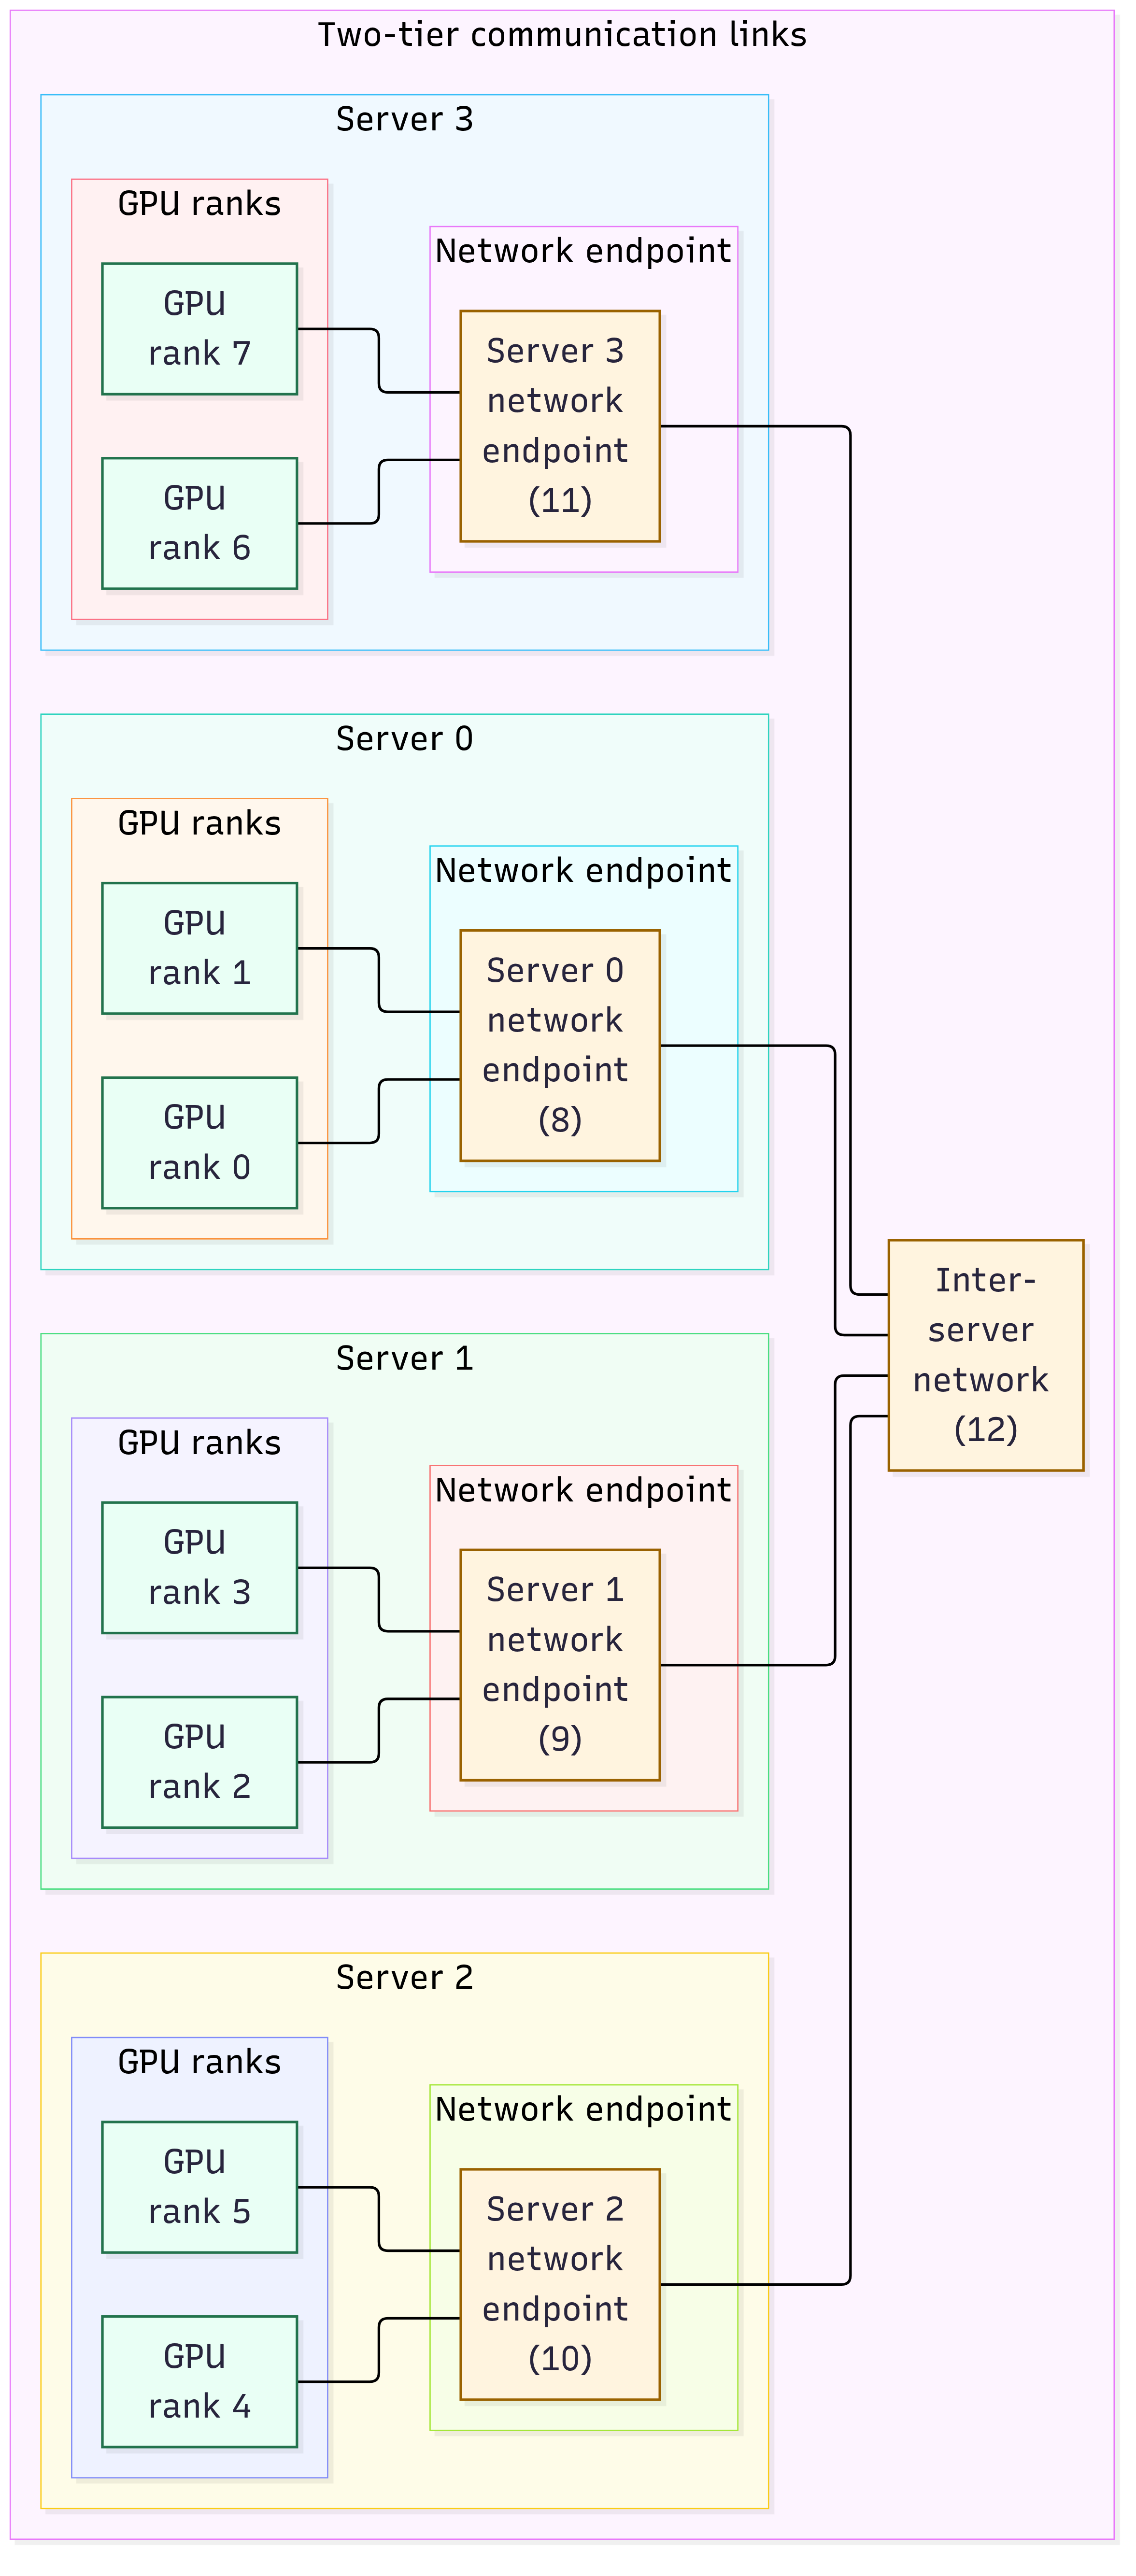
\includegraphics[width=\linewidth]{example_hotspot_links.png}
    \caption{Two-tier routed-link topology.}
  \end{subfigure}\hfill
  \begin{subfigure}[t]{0.31\textwidth}
    \centering
    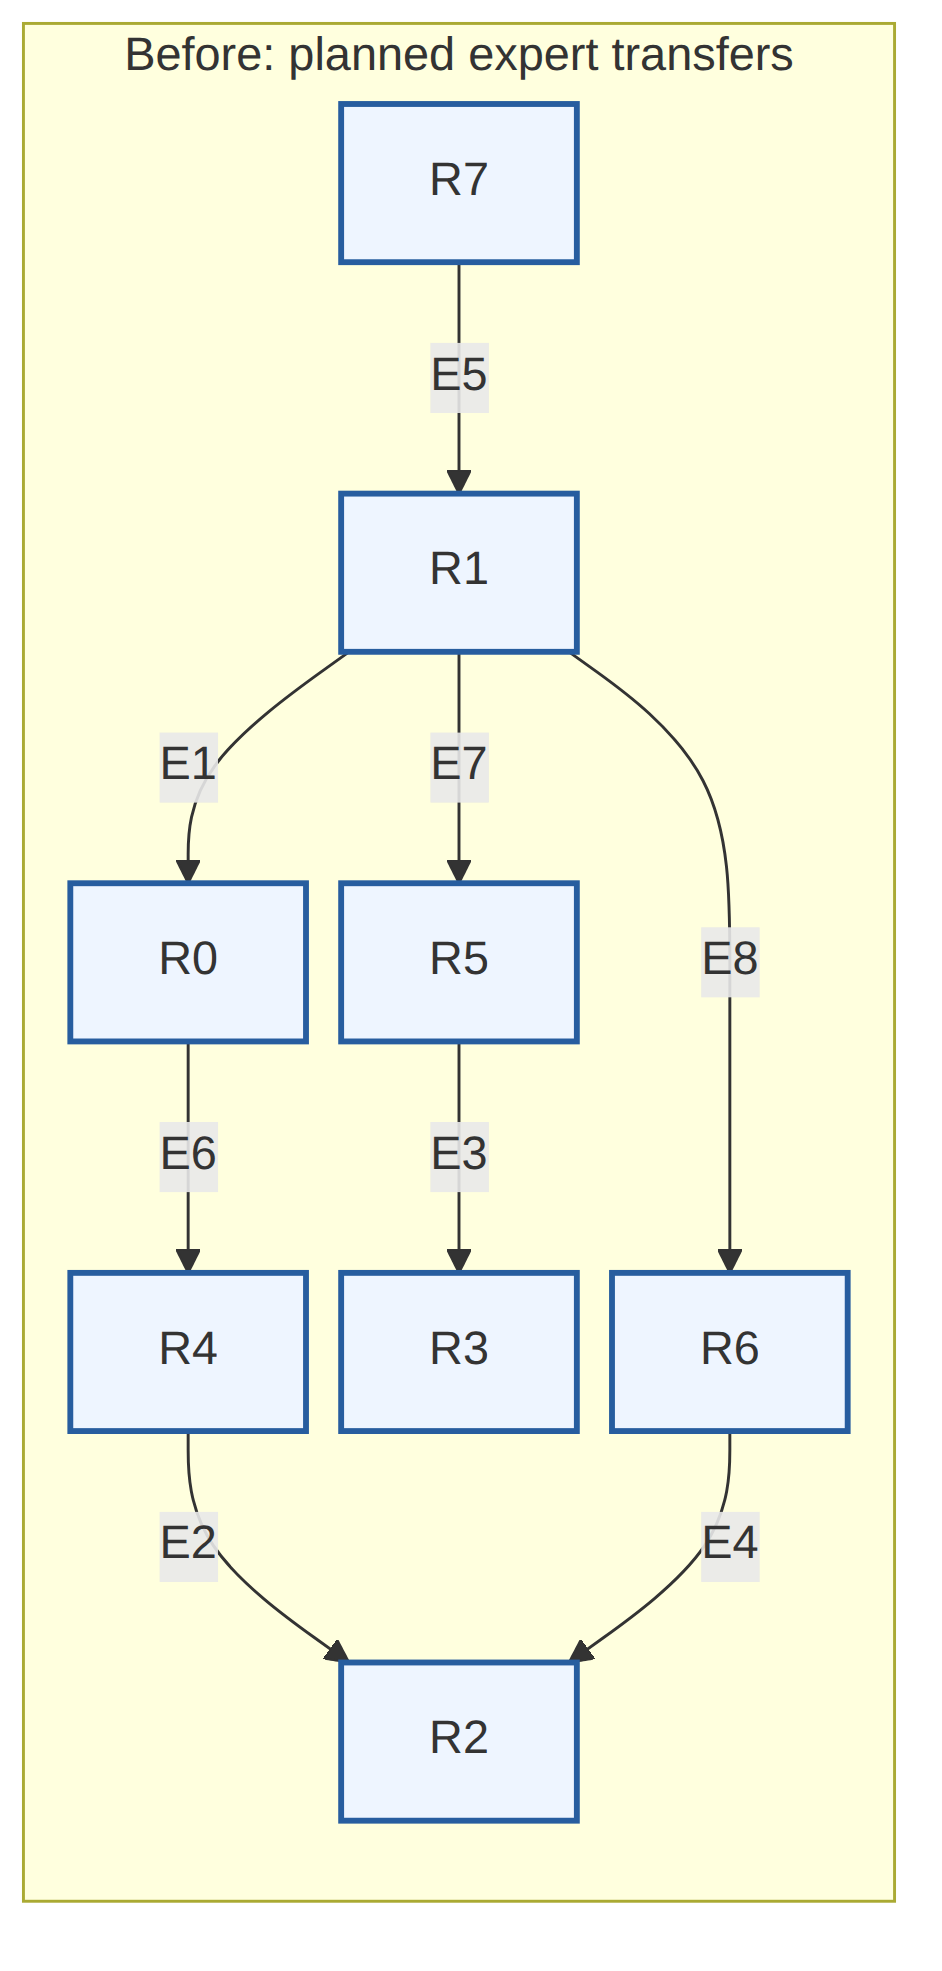
\includegraphics[width=\linewidth]{example_hotspot_before.png}
    \caption{All migrations issued together.}
  \end{subfigure}\hfill
  \begin{subfigure}[t]{0.31\textwidth}
    \centering
    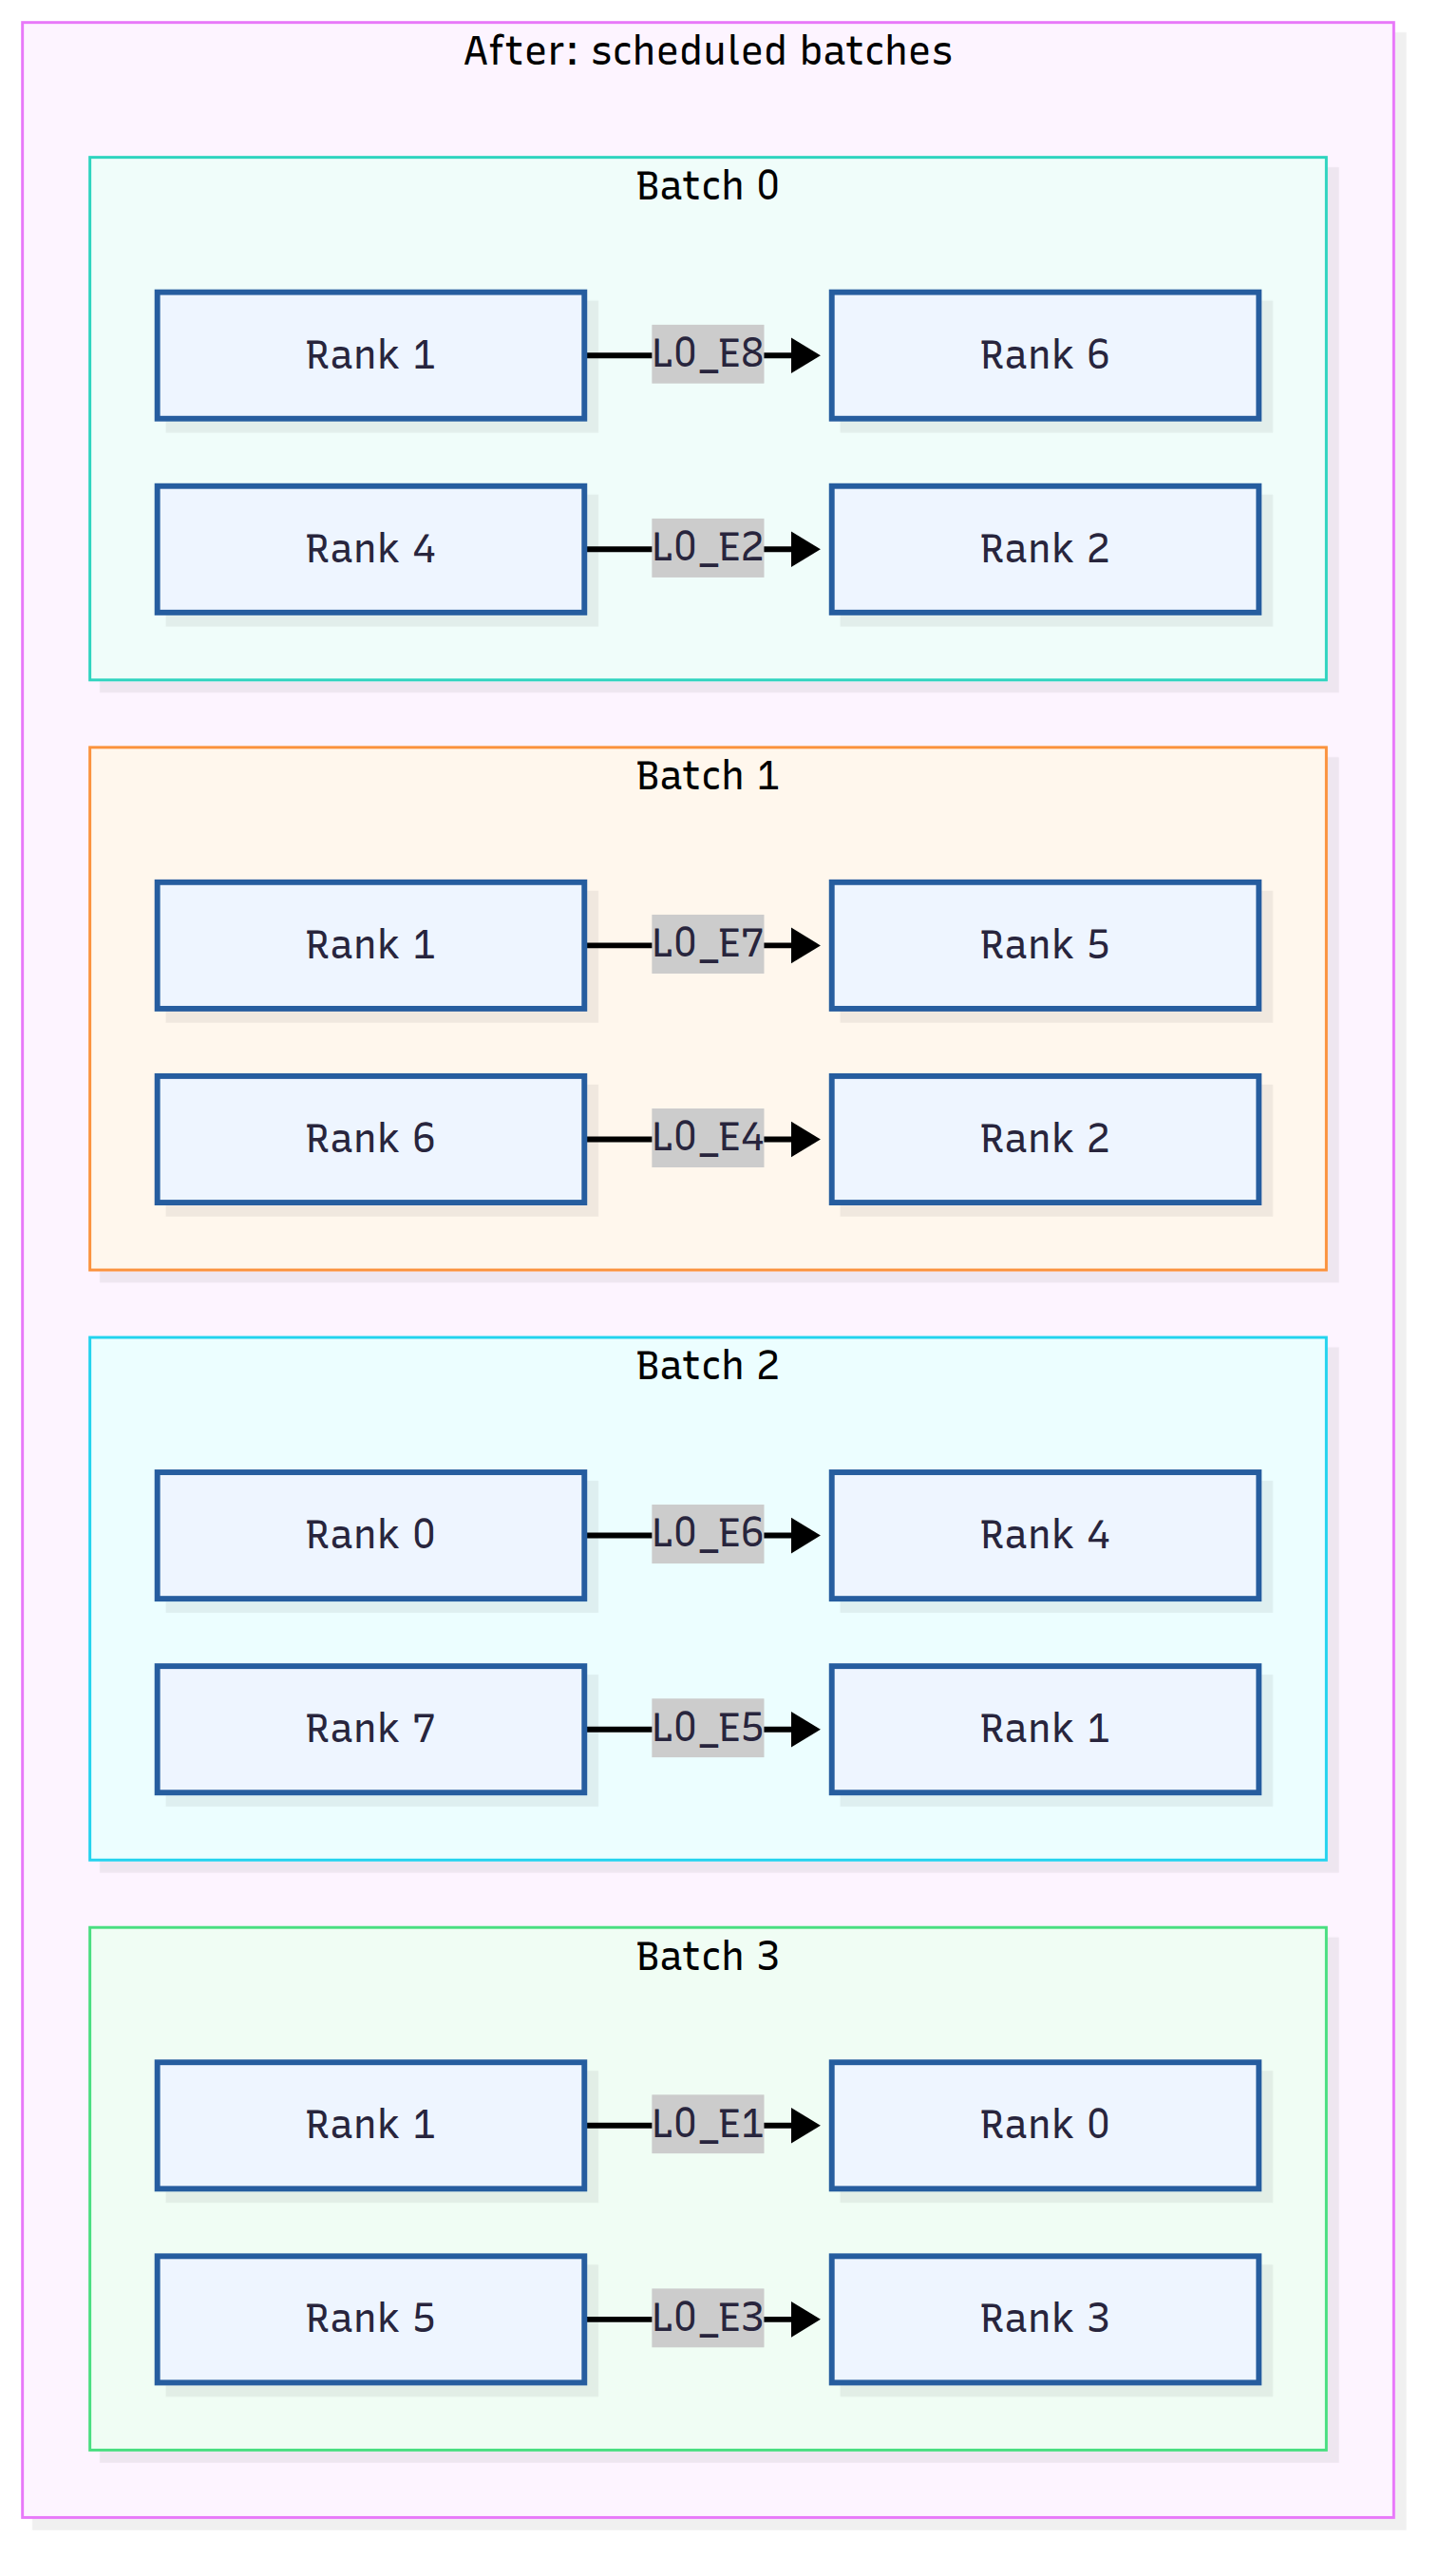
\includegraphics[width=\linewidth]{example_hotspot_after.png}
    \caption{ILP schedule split into batches.}
  \end{subfigure}
  \caption{Illustrative hotspot topology and migration schedules before and
  after contention-aware batching. The unbatched diagram remains a directed
  rank graph; only its layout is vertical.}
  \label{fig:ilp-before-after}
\end{figure}

\begin{table}[t]
  \centering
  \caption{Result of the illustrative ILP instance. Values are normalized.}
  \label{tab:ilp-result}
  \begin{tabular}{lrr}
    \toprule
    Metric & Unbatched & Constrained ILP optimum \\
    \midrule
    Modeled inference time & 4.75 & 2.25 \\
    Estimated migration time & 1.55 & 2.20 \\
    Peak link utilization & 1.50 & 0.50 \\
    Number of batches & 1 & 4 \\
    \bottomrule
  \end{tabular}
\end{table}

As shown in \cref{tab:ilp-result}, the constrained optimum reduces peak link utilization
by a factor of three and modeled inference time by more than half, but increases
estimated migration time and uses four batches. This result supplied the design
insight for the online scheduler: preserve parallelism between independent rank
pairs while explicitly limiting each rank's fan-in and fan-out within a batch.

\subsection{Why the ILP is not used online}

The optimizer is intentionally separated from the serving path. It is not an
``optimal implementation'' of EPLB: it is an exact offline reference for one
restricted mathematical formulation. First, an
online solver would add SciPy/HiGHS dependencies and variable solve latency to
a periodic control operation. Second, the latency model in
\cref{eq:slowdown} is an abstraction. Real interference depends on transport
protocols, queueing, CPU progress, message sizes, and simultaneous inference
collectives. An exact optimum of an approximate model is not necessarily a
better production choice than a conservative rule.

Third, all ranks already possess the placement maps needed to construct the
same deterministic schedule. A lightweight local algorithm avoids a new
coordination service. The ILP remains valuable for explaining the objective,
checking small instances, and motivating the endpoint constraint. The next
chapter derives the deployed algorithm from that constraint.
